% Chapter 3: ARIMA Models for Non-Stationary Data
% Comprehensive Beamer Presentation
% Bachelor program, Bucharest University of Economic Studies

\documentclass[9pt, aspectratio=169, t]{beamer}

% Ensure content fits on slides
\setbeamersize{text margin left=8mm, text margin right=8mm}

%=============================================================================
% THEME AND STYLE CONFIGURATION
%=============================================================================
\usetheme{Madrid}
\usecolortheme{seahorse}

% IDA-Inspired Color Palette
\definecolor{MainBlue}{RGB}{26, 58, 110}
\definecolor{AccentBlue}{RGB}{42, 82, 140}
\definecolor{IDAred}{RGB}{220, 53, 69}
\definecolor{DarkGray}{RGB}{51, 51, 51}
\definecolor{MediumGray}{RGB}{128, 128, 128}
\definecolor{LightGray}{RGB}{248, 248, 248}
\definecolor{VeryLightGray}{RGB}{235, 235, 235}
\definecolor{Crimson}{RGB}{220, 53, 69}
\definecolor{Forest}{RGB}{46, 125, 50}
\definecolor{Amber}{RGB}{181, 133, 63}

\setbeamercolor{palette primary}{bg=MainBlue, fg=white}
\setbeamercolor{palette secondary}{bg=MainBlue!85, fg=white}
\setbeamercolor{palette tertiary}{bg=MainBlue!70, fg=white}
\setbeamercolor{structure}{fg=MainBlue}
\setbeamercolor{title}{fg=MainBlue}
\setbeamercolor{frametitle}{fg=MainBlue, bg=white}
\setbeamercolor{block title}{bg=MainBlue, fg=white}
\setbeamercolor{block body}{bg=VeryLightGray, fg=DarkGray}
\setbeamercolor{block title alerted}{bg=Crimson, fg=white}
\setbeamercolor{block body alerted}{bg=Crimson!8, fg=DarkGray}
\setbeamercolor{block title example}{bg=Forest, fg=white}
\setbeamercolor{block body example}{bg=Forest!8, fg=DarkGray}
\setbeamercolor{item}{fg=MainBlue}

\setbeamertemplate{navigation symbols}{}

\setbeamertemplate{footline}{
    \leavevmode%
    \hbox{%
        \begin{beamercolorbox}[wd=.333333\paperwidth,ht=2.5ex,dp=1ex,center]{author in head/foot}%
            \usebeamerfont{author in head/foot}\insertshortauthor
        \end{beamercolorbox}%
        \begin{beamercolorbox}[wd=.333333\paperwidth,ht=2.5ex,dp=1ex,center]{title in head/foot}%
            \usebeamerfont{title in head/foot}\insertshorttitle
        \end{beamercolorbox}%
        \begin{beamercolorbox}[wd=.333333\paperwidth,ht=2.5ex,dp=1ex,right]{date in head/foot}%
            \usebeamerfont{date in head/foot}\insertshortdate{}\hspace*{2em}
            \insertframenumber{} / \inserttotalframenumber\hspace*{2ex}
        \end{beamercolorbox}}%
    \vskip0pt%
}

%=============================================================================
% PACKAGES
%=============================================================================
\usepackage{amsmath, amssymb, amsthm}
\usepackage{mathtools}
\usepackage{bm}
\usepackage{tikz}
\usetikzlibrary{arrows.meta, positioning, shapes, calc}
\usepackage{booktabs}
\usepackage{multirow}
\usepackage{array}
\usepackage{graphicx}
\usepackage{hyperref}
\hypersetup{colorlinks=false, pdfborder={0 0 0}}
\graphicspath{{logos/}{charts/}}

%=============================================================================
% THEOREM ENVIRONMENTS
%=============================================================================
\theoremstyle{definition}
\setbeamertemplate{theorems}[numbered]
\newtheorem{defn}{Definition}
\newtheorem{thm}{Theorem}
\newtheorem{prop}{Proposition}
\newtheorem{rmk}{Remark}

%=============================================================================
% CUSTOM COMMANDS
%=============================================================================
\newcommand{\E}{\mathbb{E}}
\newcommand{\Var}{\text{Var}}
\newcommand{\Cov}{\text{Cov}}
\newcommand{\Corr}{\text{Corr}}
\newcommand{\R}{\mathbb{R}}
\newcommand{\N}{\mathbb{N}}
\newcommand{\Z}{\mathbb{Z}}
\newcommand{\B}{\mathbf{B}}
\newcommand{\imark}{\textcolor{MainBlue}{\textbullet}}

%=============================================================================
% TITLE INFORMATION
%=============================================================================
\title[Chapter 3: ARIMA Models]{Chapter 3: ARIMA Models for Non-Stationary Data}
\subtitle{Bachelor program Faculty of Cybernetics, Statistics and Economic Informatics, Bucharest University of Economic Studies, Romania}
\author[Prof. dr. Daniel Traian Pele]{Prof. dr. Daniel Traian Pele\\[0.2cm]\footnotesize\texttt{danpele@ase.ro}}
\institute{Bucharest University of Economic Studies}
\date{Academic Year 2025--2026}

\begin{document}

%=============================================================================
% TITLE SLIDE
%=============================================================================
\begin{frame}[plain]
    \begin{tikzpicture}[remember picture, overlay]
        \node[anchor=north west] at ([xshift=0.5cm, yshift=-0.3cm]current page.north west) {
            \href{https://www.ase.ro}{\includegraphics[height=1.1cm]{ase_logo.png}}
        };
        \node[anchor=north] at ([yshift=-0.3cm]current page.north) {
            \href{https://ai4efin.ase.ro}{\includegraphics[height=1.1cm]{ai4efin_logo.png}}
        };
        \node[anchor=north east] at ([xshift=-0.5cm, yshift=-0.3cm]current page.north east) {
            \href{https://www.digital-finance-msca.com}{\includegraphics[height=1.1cm]{msca_logo.png}}
        };
    \end{tikzpicture}
    \vfill
    \begin{center}
        {\Huge\textbf{\textcolor{MainBlue}{Chapter 3: ARIMA Models}}}\\[0.5cm]
        {\Large\textcolor{MainBlue}{Non-Stationary Time Series}}
    \end{center}
    \vfill

    \begin{tikzpicture}[remember picture, overlay]
        \node[anchor=south west] at ([xshift=0.5cm, yshift=0.8cm]current page.south west) {
            \href{https://theida.net}{\includegraphics[height=0.9cm]{ida_logo.png}}
        };
        \node[anchor=south] at ([xshift=-3cm, yshift=0.8cm]current page.south) {
            \href{https://blockchain-research-center.com}{\includegraphics[height=0.9cm]{brc_logo.png}}
        };
        \node[anchor=south] at ([yshift=0.8cm]current page.south) {
            \href{https://quantinar.com}{\includegraphics[height=0.9cm]{qr_logo.png}}
        };
        \node[anchor=south] at ([xshift=3cm, yshift=0.8cm]current page.south) {
            \href{https://quantlet.com}{\includegraphics[height=0.9cm]{ql_logo.png}}
        };
        \node[anchor=south east] at ([xshift=-0.5cm, yshift=0.8cm]current page.south east) {
            \href{https://ipe.ro/new}{\includegraphics[height=0.9cm]{acad_logo.png}}
        };
    \end{tikzpicture}
\end{frame}

%=============================================================================
% TABLE OF CONTENTS
%=============================================================================
\begin{frame}{Outline}
    \vspace{-0.3cm}
    {\small
    \begin{columns}[T]
        \begin{column}{0.48\textwidth}
            \tableofcontents[sections={1-6}, hideallsubsections]
        \end{column}
        \begin{column}{0.48\textwidth}
            \tableofcontents[sections={7-11}, hideallsubsections]
        \end{column}
    \end{columns}
    }
\end{frame}

%=============================================================================
% MOTIVATION
%=============================================================================
\begin{frame}{Motivating Example: Non-Stationary Data Is Everywhere}
    \vspace{-0.3cm}
    \begin{center}
        \includegraphics[width=0.88\textwidth, height=0.62\textheight, keepaspectratio]{charts/ch3_motivation_nonstationary.pdf}
    \end{center}
    \vspace{-0.2cm}
    {\footnotesize
    \begin{itemize}
        \item Stock prices, GDP, exchange rates all exhibit \textbf{trends} or \textbf{wandering behavior}
        \item The sample mean (red line) is meaningless for a random walk
        \item Standard ARMA models \textbf{cannot} handle these series directly
    \end{itemize}
    }
\end{frame}

\begin{frame}{Real-World Applications}
    \vspace{-0.3cm}
    \begin{center}
        \includegraphics[width=0.92\textwidth, height=0.58\textheight, keepaspectratio]{charts/ch3_motivation_realworld.pdf}
    \end{center}
    \vspace{-0.2cm}
    {\footnotesize
    \begin{alertblock}{The Challenge}
        Financial and economic data are typically \textbf{integrated} (I(1) or near unit root):
        \begin{itemize}
            \item Stock prices: random walk in logs
            \item Exchange rates: random walk
            \item Interest rates: highly persistent (near unit root)
        \end{itemize}
    \end{alertblock}
    }
\end{frame}

\begin{frame}{The Solution: Differencing}
    \vspace{-0.3cm}
    \begin{center}
        \includegraphics[width=0.88\textwidth, height=0.62\textheight, keepaspectratio]{charts/ch3_motivation_differencing.pdf}
    \end{center}
    \vspace{-0.2cm}
    {\footnotesize
    \begin{exampleblock}{Key Insight}
        \textbf{Differencing} transforms a non-stationary series into a stationary one:
        $\Delta Y_t = Y_t - Y_{t-1}$. The ACF changes from slow decay to quick decay!
    \end{exampleblock}
    }
\end{frame}

\begin{frame}{What We'll Learn Today}
    \begin{block}{Core Concepts}
        \begin{enumerate}
            \item \textbf{Non-Stationarity}: Why it matters and how to detect it
            \item \textbf{Unit Root Tests}: ADF, PP, KPSS tests
            \item \textbf{Differencing}: The key transformation
            \item \textbf{ARIMA Models}: Combining differencing with ARMA
            \item \textbf{Box-Jenkins Methodology}: Identify $\to$ Estimate $\to$ Diagnose
        \end{enumerate}
    \end{block}

    \vspace{0.2cm}

    \begin{exampleblock}{By the End of This Lecture}
        You will be able to model and forecast non-stationary time series like stock prices, GDP, and exchange rates using ARIMA models.
    \end{exampleblock}
\end{frame}

%=============================================================================
% SECTION 1: NON-STATIONARITY
%=============================================================================
\section{Non-Stationarity in Time Series}

\begin{frame}{Why Non-Stationarity Matters}
    {\small
    \hfill\begin{minipage}{0.9\textwidth}
    \begin{alertblock}{The Problem}
        Many economic and financial time series are \textbf{non-stationary}:
        \begin{itemize}\setlength{\itemsep}{0pt}
            \item GDP, stock prices, exchange rates, inflation indices
            \item They exhibit trends, changing means, or growing variance
        \end{itemize}
    \end{alertblock}

    \vspace{0.1cm}

    \begin{block}{Consequences of Non-Stationarity}
        \begin{itemize}\setlength{\itemsep}{0pt}
            \item Standard ARMA models assume stationarity
            \item OLS regression with non-stationary data leads to \textbf{spurious regression}
            \item Sample moments (mean, variance, ACF) are not consistent estimators
            \item Statistical inference becomes invalid
        \end{itemize}
    \end{block}
    \end{minipage}
    }
\end{frame}

\begin{frame}{Example: US Real GDP}
    \vspace{-0.3cm}
    \begin{center}
        \includegraphics[width=0.78\textwidth, height=0.55\textheight, keepaspectratio]{charts/ch3_gdp_levels.pdf}
    \end{center}
    \vspace{-0.2cm}
    {\small
    \begin{itemize}
        \item Clear upward \textbf{trend} -- mean is not constant
        \item This is a classic example of a \textbf{non-stationary} time series
        \item We cannot apply ARMA models directly to this data
    \end{itemize}
    }
\end{frame}

\begin{frame}{Types of Non-Stationarity}
    \begin{columns}[T]
        \begin{column}{0.48\textwidth}
            \begin{block}{Deterministic Trend}
                $$Y_t = \alpha + \beta t + \varepsilon_t$$
                \begin{itemize}
                    \item Trend is a deterministic function of time
                    \item Can be removed by \textbf{detrending}
                    \item Shocks have temporary effects
                \end{itemize}
            \end{block}
        \end{column}
        \begin{column}{0.48\textwidth}
            \begin{block}{Stochastic Trend (Unit Root)}
                $$Y_t = Y_{t-1} + \varepsilon_t$$
                \begin{itemize}
                    \item Random walk process
                    \item Must be removed by \textbf{differencing}
                    \item Shocks have permanent effects
                \end{itemize}
            \end{block}
        \end{column}
    \end{columns}

    \vspace{0.5cm}

    \begin{alertblock}{Key Distinction}
        Correct identification is crucial: detrending a unit root process or differencing a trend-stationary process both lead to misspecification!
    \end{alertblock}
\end{frame}

\begin{frame}{Visualizing the Difference}
    \vspace{-0.3cm}
    \begin{center}
        \includegraphics[width=0.82\textwidth, height=0.58\textheight, keepaspectratio]{charts/ch3_trend_comparison.pdf}
    \end{center}
    \vspace{-0.2cm}
    {\footnotesize
    \begin{itemize}
        \item \textbf{Left}: Deterministic trend -- deviations from trend are temporary
        \item \textbf{Right}: Stochastic trend -- shocks accumulate permanently
        \item Both look similar, but require \textbf{different} treatments!
    \end{itemize}
    }
\end{frame}

\begin{frame}{The Random Walk Process}
    {\small
    \hfill\begin{minipage}{0.9\textwidth}
    \begin{defn}[Random Walk]
        A \textbf{random walk} is defined as:
        $$Y_t = Y_{t-1} + \varepsilon_t, \quad \varepsilon_t \sim WN(0, \sigma^2)$$
        With initial condition $Y_0 = 0$, we have: $Y_t = \sum_{i=1}^{t} \varepsilon_i$
    \end{defn}

    \vspace{0.1cm}

    \begin{block}{Properties of Random Walk}
        \begin{itemize}\setlength{\itemsep}{0pt}
            \item $\E[Y_t] = 0$ (constant mean)
            \item $\Var(Y_t) = t\sigma^2$ (variance grows with time!)
            \item $\Cov(Y_t, Y_{t-k}) = (t-k)\sigma^2$ for $k \leq t$
            \item ACF: $\rho_k = \sqrt{\frac{t-k}{t}} \to 1$ as $t \to \infty$
        \end{itemize}
    \end{block}
    \end{minipage}
    }
\end{frame}

\begin{frame}{Random Walk with Drift}
    {\small
    \hfill\begin{minipage}{0.9\textwidth}
    \begin{defn}[Random Walk with Drift]
        A random walk with drift includes a constant term:
        $$Y_t = \mu + Y_{t-1} + \varepsilon_t$$
        Equivalently: $Y_t = Y_0 + \mu t + \sum_{i=1}^{t} \varepsilon_i$
    \end{defn}

    \vspace{0.1cm}

    \begin{block}{Properties}
        \begin{itemize}\setlength{\itemsep}{0pt}
            \item $\E[Y_t] = Y_0 + \mu t$ (mean grows linearly)
            \item $\Var(Y_t) = t\sigma^2$ (variance still grows)
            \item The drift $\mu$ creates an upward or downward trend
            \item Still non-stationary despite having a ``trend''
        \end{itemize}
    \end{block}
    \end{minipage}
    }
\end{frame}

\begin{frame}{Simulating Random Walks}
    \vspace{-0.3cm}
    \begin{center}
        \includegraphics[width=0.82\textwidth, height=0.58\textheight, keepaspectratio]{charts/ch3_random_walk.pdf}
    \end{center}
    \vspace{-0.2cm}
    {\footnotesize
    \begin{itemize}
        \item \textbf{Left}: Pure random walks -- no drift, wander unpredictably
        \item \textbf{Right}: Random walks with drift -- upward trend on average
        \item Each path is unique; uncertainty grows over time
    \end{itemize}
    }
\end{frame}

\begin{frame}{Variance Growth: Why Random Walks Are Non-Stationary}
    \vspace{-0.3cm}
    \begin{center}
        \includegraphics[width=0.82\textwidth, height=0.58\textheight, keepaspectratio]{charts/ch3_variance_growth.pdf}
    \end{center}
    \vspace{-0.2cm}
    {\footnotesize
    \begin{itemize}
        \item \textbf{Left}: Fan of paths shows uncertainty growing over time
        \item \textbf{Right}: Variance grows linearly: $\Var(Y_t) = t\sigma^2$
        \item This violates stationarity (variance should be constant)
    \end{itemize}
    }
\end{frame}

\begin{frame}{Integrated Processes}
    {\small
    \hfill\begin{minipage}{0.9\textwidth}
    \begin{defn}[Integrated Process of Order $d$]
        A time series $\{Y_t\}$ is \textbf{integrated of order $d$}, written $Y_t \sim I(d)$, if:
        \begin{itemize}\setlength{\itemsep}{0pt}
            \item $Y_t$ is non-stationary
            \item $(1-L)^d Y_t = \Delta^d Y_t$ is stationary
            \item $(1-L)^{d-1} Y_t$ is still non-stationary
        \end{itemize}
    \end{defn}

    \vspace{0.1cm}

    \begin{exampleblock}{Common Cases}
        \begin{itemize}\setlength{\itemsep}{0pt}
            \item $I(0)$: Stationary process (e.g., ARMA)
            \item $I(1)$: First difference is stationary (most common for economic data)
            \item $I(2)$: Second difference is stationary (less common)
        \end{itemize}
    \end{exampleblock}
    \end{minipage}
    }
\end{frame}

%=============================================================================
% SECTION 2: DIFFERENCING
%=============================================================================
\section{Differencing and the Difference Operator}

\begin{frame}{The Difference Operator}
    {\small
    \hfill\begin{minipage}{0.9\textwidth}
    \begin{defn}[First Difference]
        The \textbf{first difference operator} $\Delta$ is defined as:
        $\Delta Y_t = Y_t - Y_{t-1} = (1-L)Y_t$, where $L$ is the lag operator ($LY_t = Y_{t-1}$).
    \end{defn}

    \vspace{0.1cm}

    \begin{block}{Higher-Order Differences}
        \begin{itemize}\setlength{\itemsep}{0pt}
            \item Second difference: $\Delta^2 Y_t = \Delta(\Delta Y_t) = (1-L)^2 Y_t$
            \item $\Delta^2 Y_t = Y_t - 2Y_{t-1} + Y_{t-2}$
            \item $d$-th difference: $\Delta^d Y_t = (1-L)^d Y_t$
        \end{itemize}
    \end{block}

    \vspace{0.1cm}

    \begin{alertblock}{Key Result}
        If $Y_t \sim I(d)$, then $\Delta^d Y_t \sim I(0)$ (stationary).
    \end{alertblock}
    \end{minipage}
    }
\end{frame}

\begin{frame}{Example: Differencing a Random Walk}
    {\small
    \hfill\begin{minipage}{0.9\textwidth}
    \begin{exampleblock}{Random Walk to White Noise}
        Let $Y_t = Y_{t-1} + \varepsilon_t$ (random walk). Taking the first difference:
        $$\Delta Y_t = Y_t - Y_{t-1} = \varepsilon_t$$
        The first difference is white noise -- a stationary process!
    \end{exampleblock}

    \vspace{0.1cm}

    \begin{block}{Interpretation}
        \begin{itemize}\setlength{\itemsep}{0pt}
            \item A random walk is $I(1)$
            \item One difference transforms it to $I(0)$
            \item The ``changes'' in a random walk are stationary
        \end{itemize}
    \end{block}
    \end{minipage}
    }
\end{frame}

\begin{frame}{ACF Diagnostic: Detecting Non-Stationarity}
    \vspace{-0.3cm}
    \begin{center}
        \includegraphics[width=0.82\textwidth, height=0.6\textheight, keepaspectratio]{charts/ch3_acf_nonstationary.pdf}
    \end{center}
    \vspace{-0.2cm}
    {\footnotesize
    \begin{itemize}
        \item \textbf{Top}: Random walk ACF decays very slowly $\Rightarrow$ unit root
        \item \textbf{Bottom}: After differencing, ACF cuts off $\Rightarrow$ stationary
    \end{itemize}
    }
\end{frame}

\begin{frame}{Differencing in Practice: GDP Example}
    \vspace{-0.3cm}
    \begin{center}
        \includegraphics[width=0.82\textwidth, height=0.55\textheight, keepaspectratio]{charts/ch3_differencing.pdf}
    \end{center}
    \vspace{-0.2cm}
    {\footnotesize
    \begin{itemize}
        \item \textbf{Left}: GDP in levels -- clear upward trend (non-stationary)
        \item \textbf{Right}: GDP growth rate (log difference) -- fluctuates around mean (stationary)
        \item Differencing removes the trend and achieves stationarity
    \end{itemize}
    }
\end{frame}

\begin{frame}{Overdifferencing}
    {\small
    \hfill\begin{minipage}{0.9\textwidth}
    \begin{alertblock}{Warning: Overdifferencing}
        Differencing more than necessary introduces problems:
        \begin{itemize}\setlength{\itemsep}{0pt}
            \item Creates artificial negative autocorrelation
            \item Inflates variance
            \item Loses information
        \end{itemize}
    \end{alertblock}

    \vspace{0.1cm}

    \begin{exampleblock}{Example}
        If $Y_t \sim I(1)$, then $\Delta Y_t \sim I(0)$. But if we difference again:
        $$\Delta^2 Y_t = \Delta Y_t - \Delta Y_{t-1} = \varepsilon_t - \varepsilon_{t-1}$$
        This is an MA(1) with $\theta = 1$ (non-invertible boundary)!
    \end{exampleblock}
    \end{minipage}
    }
\end{frame}

%=============================================================================
% SECTION 3: ARIMA MODELS
%=============================================================================
\section{ARIMA(p,d,q) Models}

\begin{frame}{Definition of ARIMA}
    {\small
    \hfill\begin{minipage}{0.9\textwidth}
    \begin{defn}[ARIMA(p,d,q)]
        A time series $\{Y_t\}$ follows an \textbf{ARIMA(p,d,q)} process if:
        $$\phi(L)(1-L)^d Y_t = c + \theta(L)\varepsilon_t$$
        where:
        \begin{itemize}\setlength{\itemsep}{0pt}
            \item $\phi(L) = 1 - \phi_1 L - \phi_2 L^2 - \cdots - \phi_p L^p$ (AR polynomial)
            \item $\theta(L) = 1 + \theta_1 L + \theta_2 L^2 + \cdots + \theta_q L^q$ (MA polynomial)
            \item $d$ is the order of integration (number of differences)
            \item $\varepsilon_t \sim WN(0, \sigma^2)$
        \end{itemize}
    \end{defn}
    \end{minipage}
    }
\end{frame}

\begin{frame}{ARIMA Components}
    \begin{center}
        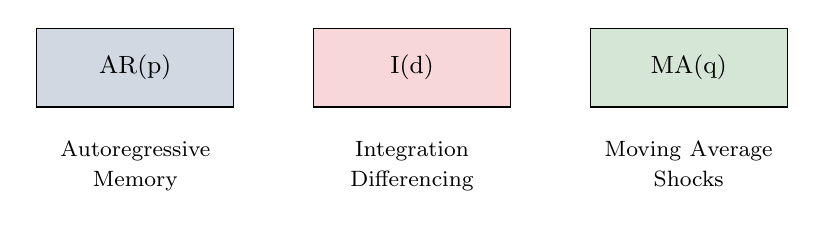
\begin{tikzpicture}[node distance=2cm, every node/.style={font=\small}]
            \node[draw, rectangle, fill=MainBlue!20, minimum width=2.5cm, minimum height=1cm] (AR) {AR(p)};
            \node[draw, rectangle, fill=Crimson!20, minimum width=2.5cm, minimum height=1cm, right=1cm of AR] (I) {I(d)};
            \node[draw, rectangle, fill=Forest!20, minimum width=2.5cm, minimum height=1cm, right=1cm of I] (MA) {MA(q)};

            \node[below=0.3cm of AR, text width=2.5cm, align=center] {\footnotesize Autoregressive\\Memory};
            \node[below=0.3cm of I, text width=2.5cm, align=center] {\footnotesize Integration\\Differencing};
            \node[below=0.3cm of MA, text width=2.5cm, align=center] {\footnotesize Moving Average\\Shocks};
        \end{tikzpicture}
    \end{center}

    \vspace{0.2cm}

    {\small
    \begin{block}{Special Cases}
        \begin{itemize}\setlength{\itemsep}{0pt}
            \item ARIMA(p,0,q) = ARMA(p,q) -- stationary
            \item ARIMA(0,1,0) = Random walk
            \item ARIMA(0,1,1) = IMA(1,1) -- exponential smoothing
            \item ARIMA(1,1,0) = ARI(1,1) -- differenced AR(1)
        \end{itemize}
    \end{block}
    }
\end{frame}

\begin{frame}{ARIMA(1,1,0) Example}
    {\small
    \hfill\begin{minipage}{0.9\textwidth}
    \begin{exampleblock}{ARI(1,1) Model}
        $$\Delta Y_t = c + \phi_1 \Delta Y_{t-1} + \varepsilon_t$$
        Equivalently: $(1-\phi_1 L)(1-L)Y_t = c + \varepsilon_t$
    \end{exampleblock}

    \vspace{0.1cm}

    \begin{block}{Interpretation}
        \begin{itemize}\setlength{\itemsep}{0pt}
            \item The \textbf{changes} in $Y_t$ follow an AR(1) process
            \item If $|\phi_1| < 1$, the changes are stationary
            \item $Y_t$ itself has a stochastic trend
            \item Common model for many economic time series
        \end{itemize}
    \end{block}
    \end{minipage}
    }
\end{frame}

\begin{frame}{ARIMA(0,1,1) Example}
    {\small
    \hfill\begin{minipage}{0.9\textwidth}
    \begin{exampleblock}{IMA(1,1) Model}
        $$\Delta Y_t = c + \varepsilon_t + \theta_1 \varepsilon_{t-1}$$
        Equivalently: $(1-L)Y_t = c + (1+\theta_1 L)\varepsilon_t$
    \end{exampleblock}

    \vspace{0.1cm}

    \begin{block}{Connection to Exponential Smoothing}
        The IMA(1,1) model is equivalent to \textbf{simple exponential smoothing}:
        $$\hat{Y}_{t+1} = \alpha Y_t + (1-\alpha)\hat{Y}_t$$
        where $\alpha = 1 + \theta_1$ (for $-1 < \theta_1 < 0$).
    \end{block}
    \end{minipage}
    }
\end{frame}

\begin{frame}{The Role of the Constant in ARIMA}
    {\small
    \hfill\begin{minipage}{0.9\textwidth}
    \begin{block}{Constant Term in ARIMA(p,d,q)}
        When $d > 0$, the constant $c$ has a different interpretation:
        $\phi(L)(1-L)^d Y_t = c + \theta(L)\varepsilon_t$
    \end{block}

    \vspace{0.1cm}

    \begin{alertblock}{Important Implications}
        \begin{itemize}\setlength{\itemsep}{0pt}
            \item For $d=1$: $c$ represents the \textbf{drift} (average change): $\E[\Delta Y_t] = \frac{c}{1-\phi_1-\cdots-\phi_p}$
            \item For $d=2$: $c$ affects the \textbf{curvature} of the trend
            \item Often $c=0$ is assumed when $d \geq 1$
        \end{itemize}
    \end{alertblock}
    \end{minipage}
    }
\end{frame}

%=============================================================================
% SECTION 4: UNIT ROOT TESTS
%=============================================================================
\section{Unit Root Tests}

\begin{frame}{Testing for Unit Roots}
    {\small
    \hfill\begin{minipage}{0.9\textwidth}
    \begin{block}{Why Test?}
        Before fitting an ARIMA model, we need to determine:
        \begin{enumerate}\setlength{\itemsep}{0pt}
            \item Is the series stationary? (Is $d=0$?)
            \item If not, how many differences are needed? (What is $d$?)
        \end{enumerate}
    \end{block}

    \vspace{0.1cm}

    \begin{block}{Common Unit Root Tests}
        \begin{itemize}\setlength{\itemsep}{0pt}
            \item \textbf{Dickey-Fuller (DF)} and \textbf{Augmented Dickey-Fuller (ADF)}
            \item \textbf{Phillips-Perron (PP)}
            \item \textbf{KPSS} (stationarity test -- reversed null hypothesis)
        \end{itemize}
    \end{block}
    \end{minipage}
    }
\end{frame}

\begin{frame}{The Dickey-Fuller Test}
    {\small
    \hfill\begin{minipage}{0.9\textwidth}
    \begin{block}{Setup}
        Consider the AR(1) model: $Y_t = \phi Y_{t-1} + \varepsilon_t$. Subtract $Y_{t-1}$:
        $\Delta Y_t = (\phi - 1)Y_{t-1} + \varepsilon_t = \gamma Y_{t-1} + \varepsilon_t$, where $\gamma = \phi - 1$.
    \end{block}

    \vspace{0.1cm}

    \begin{block}{Hypotheses}
        \begin{itemize}\setlength{\itemsep}{0pt}
            \item $H_0$: $\gamma = 0$ (unit root, $\phi = 1$, non-stationary)
            \item $H_1$: $\gamma < 0$ (stationary, $|\phi| < 1$)
        \end{itemize}
    \end{block}

    \vspace{0.1cm}

    \begin{alertblock}{Key Issue}
        Under $H_0$, the $t$-statistic does \textbf{not} follow a standard $t$-distribution! Must use Dickey-Fuller critical values.
    \end{alertblock}
    \end{minipage}
    }
\end{frame}

\begin{frame}{Dickey-Fuller Test Variants}
    {\small
    \hfill\begin{minipage}{0.9\textwidth}
    \begin{block}{Three Specifications}
        \begin{enumerate}\setlength{\itemsep}{0pt}
            \item \textbf{No constant, no trend}: $\Delta Y_t = \gamma Y_{t-1} + \varepsilon_t$
            \item \textbf{With constant (drift)}: $\Delta Y_t = \alpha + \gamma Y_{t-1} + \varepsilon_t$
            \item \textbf{With constant and trend}: $\Delta Y_t = \alpha + \beta t + \gamma Y_{t-1} + \varepsilon_t$
        \end{enumerate}
    \end{block}

    \vspace{0.1cm}

    \begin{alertblock}{Choosing the Right Specification}
        \begin{itemize}\setlength{\itemsep}{0pt}
            \item Examine the data: does it have a visible trend?
            \item Including unnecessary terms reduces power
            \item Excluding necessary terms leads to incorrect inference
        \end{itemize}
    \end{alertblock}
    \end{minipage}
    }
\end{frame}

\begin{frame}{Augmented Dickey-Fuller (ADF) Test}
    \vspace{-0.2cm}
    {\small
    \begin{block}{The Problem with Simple DF}
        If AR dynamics beyond AR(1) exist, DF residuals will be autocorrelated.
    \end{block}

    \vspace{0.1cm}

    \begin{defn}[ADF Test]
        Add lagged differences: $\Delta Y_t = \alpha + \beta t + \gamma Y_{t-1} + \sum_{j=1}^{k} \delta_j \Delta Y_{t-j} + \varepsilon_t$

        Test $H_0: \gamma = 0$ using ADF critical values.
    \end{defn}

    \vspace{0.1cm}

    \begin{block}{Choosing Lag Length $k$}
        \begin{itemize}
            \item Use information criteria (AIC, BIC)
            \item Start with $k_{max}$, reduce until last lag significant
        \end{itemize}
    \end{block}
    }
\end{frame}

\begin{frame}{ADF Test Critical Values}
    \vspace{-0.2cm}
    {\small
    \begin{table}
        \centering
        \begin{tabular}{lccc}
            \toprule
            \textbf{Model} & \textbf{1\%} & \textbf{5\%} & \textbf{10\%} \\
            \midrule
            No constant, no trend & $-2.58$ & $-1.95$ & $-1.62$ \\
            With constant & $-3.43$ & $-2.86$ & $-2.57$ \\
            With constant and trend & $-3.96$ & $-3.41$ & $-3.13$ \\
            \bottomrule
        \end{tabular}
    \end{table}
    }
    \vspace{-0.1cm}
    \begin{block}{Decision Rule}
        {\small
        \begin{itemize}
            \item Test statistic $<$ critical value $\Rightarrow$ Reject $H_0$ (stationary)
            \item Test statistic $\geq$ critical value $\Rightarrow$ Fail to reject (unit root)
        \end{itemize}
        }
    \end{block}
\end{frame}

\begin{frame}{The Phillips-Perron (PP) Test}
    {\small
    \hfill\begin{minipage}{0.9\textwidth}
    \begin{block}{Motivation}
        Like ADF, tests $H_0$: Unit root vs $H_1$: Stationary, but uses a \textbf{non-parametric correction} for serial correlation instead of adding lagged differences.
    \end{block}

    \begin{block}{Test Statistic}
        The PP test modifies the DF $t$-statistic:
        $$Z_t = t_{\hat{\gamma}} \cdot \sqrt{\frac{\hat{\sigma}^2}{\hat{\lambda}^2}} - \frac{T(\hat{\lambda}^2 - \hat{\sigma}^2)(se(\hat{\gamma}))}{2\hat{\lambda}^2 \cdot s}$$
        where $\hat{\lambda}^2$ is a consistent estimate of the long-run variance using Newey-West.
    \end{block}

    \begin{exampleblock}{Advantages over ADF}
        \begin{itemize}\setlength{\itemsep}{0pt}
            \item Robust to heteroskedasticity and serial correlation
            \item No need to select lag length (uses bandwidth instead)
        \end{itemize}
    \end{exampleblock}
    \end{minipage}
    }
\end{frame}

\begin{frame}{The KPSS Test}
    \vspace{-0.2cm}
    {\small
    \hfill\begin{minipage}{0.9\textwidth}
    \begin{block}{Reversed Hypotheses}
        Unlike ADF: $H_0$: Stationary \quad vs \quad $H_1$: Unit root
    \end{block}

    \vspace{0.1cm}

    \begin{block}{KPSS Procedure}
        Decompose: $Y_t = \xi t + r_t + \varepsilon_t$ where $r_t = r_{t-1} + u_t$.
        Test whether $\Var(u_t) = 0$.
    \end{block}

    \vspace{0.1cm}

    \begin{exampleblock}{Complementary Use with ADF}
        \begin{itemize}
            \item ADF rejects, KPSS doesn't $\Rightarrow$ Stationary
            \item ADF doesn't reject, KPSS rejects $\Rightarrow$ Unit root
            \item Both reject or neither $\Rightarrow$ Inconclusive
        \end{itemize}
    \end{exampleblock}
    \end{minipage}
    }
\end{frame}

%=============================================================================
% SECTION 5: MODEL IDENTIFICATION
%=============================================================================
\section{ARIMA Model Identification}

\begin{frame}{The Box-Jenkins Methodology}
    \begin{center}
        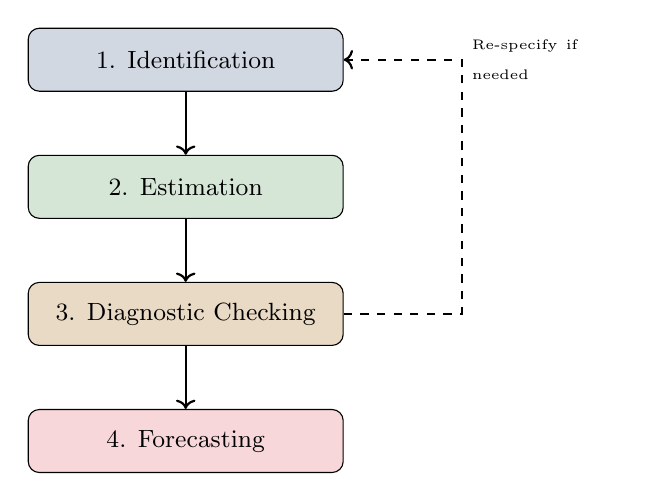
\begin{tikzpicture}[node distance=1.5cm, every node/.style={font=\small}]
            \node[draw, rectangle, rounded corners, fill=MainBlue!20, minimum width=4cm, minimum height=0.8cm] (id) {1. Identification};
            \node[draw, rectangle, rounded corners, fill=Forest!20, minimum width=4cm, minimum height=0.8cm, below=0.8cm of id] (est) {2. Estimation};
            \node[draw, rectangle, rounded corners, fill=Amber!30, minimum width=4cm, minimum height=0.8cm, below=0.8cm of est] (diag) {3. Diagnostic Checking};
            \node[draw, rectangle, rounded corners, fill=Crimson!20, minimum width=4cm, minimum height=0.8cm, below=0.8cm of diag] (fore) {4. Forecasting};

            \draw[->, thick] (id) -- (est);
            \draw[->, thick] (est) -- (diag);
            \draw[->, thick] (diag) -- (fore);
            \draw[->, thick, dashed] (diag.east) -- ++(1.5,0) |- (id.east) node[midway, right, text width=2cm] {\tiny Re-specify if needed};
        \end{tikzpicture}
    \end{center}
\end{frame}

\begin{frame}{Step 1: Determining $d$}
    {\small
    \hfill\begin{minipage}{0.9\textwidth}
    \begin{block}{Procedure}
        \begin{enumerate}\setlength{\itemsep}{0pt}
            \item Plot the time series -- look for trends, changing variance
            \item Examine ACF -- slow decay suggests non-stationarity
            \item Apply unit root tests (ADF, KPSS)
            \item If non-stationary, difference and repeat
        \end{enumerate}
    \end{block}

    \vspace{0.1cm}

    \begin{exampleblock}{Practical Guidelines}
        \begin{itemize}\setlength{\itemsep}{0pt}
            \item Most economic series: $d = 1$ is sufficient
            \item Rarely need $d > 2$
            \item If ACF of $\Delta Y_t$ still decays slowly, try $d = 2$
            \item Watch for overdifferencing (ACF with $\rho_1 \approx -0.5$)
        \end{itemize}
    \end{exampleblock}
    \end{minipage}
    }
\end{frame}

\begin{frame}{Step 2: Determining $p$ and $q$}
    {\small
    \begin{block}{After Differencing}
        Once $W_t = \Delta^d Y_t$ is stationary, use ACF/PACF to identify ARMA($p$,$q$):
    \end{block}

    \vspace{0.1cm}

    \begin{table}
        \centering
        \begin{tabular}{lcc}
            \toprule
            \textbf{Model} & \textbf{ACF} & \textbf{PACF} \\
            \midrule
            AR($p$) & Decays exponentially & Cuts off after lag $p$ \\
            MA($q$) & Cuts off after lag $q$ & Decays exponentially \\
            ARMA($p$,$q$) & Decays & Decays \\
            \bottomrule
        \end{tabular}
    \end{table}

    \vspace{0.1cm}

    \begin{block}{Information Criteria}
        When patterns are unclear, compare models using:
        \begin{itemize}\setlength{\itemsep}{0pt}
            \item AIC = $-2\ln(L) + 2k$; \quad BIC = $-2\ln(L) + k\ln(n)$
        \end{itemize}
        Lower is better. BIC penalizes complexity more.
    \end{block}
    }
\end{frame}

\begin{frame}{Auto-ARIMA Algorithms}
    {\small
    \hfill\begin{minipage}{0.9\textwidth}
    \begin{block}{Automated Model Selection}
        Modern software can automatically select $(p,d,q)$:
        \begin{itemize}\setlength{\itemsep}{0pt}
            \item Python: \texttt{pmdarima.auto\_arima()}
            \item R: \texttt{forecast::auto.arima()}
        \end{itemize}
    \end{block}

    \vspace{0.1cm}

    \begin{block}{How Auto-ARIMA Works}
        \begin{enumerate}\setlength{\itemsep}{0pt}
            \item Use unit root tests to determine $d$
            \item Fit models for various $(p,q)$ combinations
            \item Select model with lowest AIC/BIC
            \item Optionally use stepwise search for efficiency
        \end{enumerate}
    \end{block}

    \vspace{0.1cm}

    \begin{alertblock}{Caution}
        Automated selection is helpful but not infallible. Always check diagnostics!
    \end{alertblock}
    \end{minipage}
    }
\end{frame}

%=============================================================================
% SECTION 6: ESTIMATION
%=============================================================================
\section{ARIMA Estimation}

\begin{frame}{Estimation Methods}
    {\small
    \hfill\begin{minipage}{0.9\textwidth}
    \begin{block}{Maximum Likelihood Estimation (MLE)}
        The standard approach for ARIMA:
        \begin{itemize}\setlength{\itemsep}{0pt}
            \item Assumes $\varepsilon_t \sim N(0, \sigma^2)$
            \item Maximizes the likelihood function
            \item Provides consistent, efficient estimators
            \item Yields standard errors for inference
        \end{itemize}
    \end{block}

    \vspace{0.1cm}

    \begin{block}{Conditional vs Exact MLE}
        \begin{itemize}\setlength{\itemsep}{0pt}
            \item \textbf{Conditional MLE}: Conditions on initial values
            \item \textbf{Exact MLE}: Treats initial values as unknown
            \item Difference diminishes as sample size grows
        \end{itemize}
    \end{block}
    \end{minipage}
    }
\end{frame}

\begin{frame}{Parameter Constraints}
    {\small
    \hfill\begin{minipage}{0.9\textwidth}
    \begin{alertblock}{Stationarity and Invertibility}
        The estimated ARIMA model should satisfy:
        \begin{itemize}\setlength{\itemsep}{0pt}
            \item \textbf{AR stationarity}: Roots of $\phi(z) = 0$ outside unit circle
            \item \textbf{MA invertibility}: Roots of $\theta(z) = 0$ outside unit circle
        \end{itemize}
    \end{alertblock}

    \vspace{0.1cm}

    \begin{block}{Checking in Practice}
        Most software reports:
        \begin{itemize}\setlength{\itemsep}{0pt}
            \item Estimated coefficients with standard errors
            \item Roots of AR and MA polynomials
            \item Warning if near-unit-root detected
        \end{itemize}
    \end{block}
    \end{minipage}
    }
\end{frame}

%=============================================================================
% SECTION 7: DIAGNOSTICS
%=============================================================================
\section{Diagnostic Checking}

\begin{frame}{Residual Analysis}
    {\small
    \hfill\begin{minipage}{0.9\textwidth}
    \begin{block}{What to Check}
        If the model is correct, residuals $\hat{\varepsilon}_t$ should be white noise:
        \begin{enumerate}\setlength{\itemsep}{0pt}
            \item Zero mean
            \item Constant variance
            \item No autocorrelation
            \item (Optional) Normality
        \end{enumerate}
    \end{block}

    \vspace{0.1cm}

    \begin{block}{Diagnostic Tools}
        \begin{itemize}\setlength{\itemsep}{0pt}
            \item \textbf{Residual ACF/PACF}: Should show no significant spikes
            \item \textbf{Ljung-Box test}: Tests for autocorrelation at multiple lags
            \item \textbf{Q-Q plot}: Checks normality assumption
            \item \textbf{Residual vs fitted}: Checks for heteroskedasticity
        \end{itemize}
    \end{block}
    \end{minipage}
    }
\end{frame}

\begin{frame}{The Ljung-Box Test}
    {\small
    \hfill\begin{minipage}{0.9\textwidth}
    \begin{defn}[Ljung-Box Q Statistic]
        $Q(m) = n(n+2) \sum_{k=1}^{m} \frac{\hat{\rho}_k^2}{n-k}$. Under $H_0$ (no autocorrelation): $Q(m) \sim \chi^2(m-p-q)$
    \end{defn}

    \vspace{0.1cm}

    \begin{block}{Usage}
        \begin{itemize}\setlength{\itemsep}{0pt}
            \item Choose $m \approx \ln(n)$ or $m = 10$ for quarterly, $m = 20$ for monthly
            \item Degrees of freedom adjusted for estimated parameters
            \item Reject if $Q(m)$ exceeds critical value
        \end{itemize}
    \end{block}

    \vspace{0.1cm}

    \begin{alertblock}{If Test Fails}
        Consider adding AR or MA terms, or check for structural breaks.
    \end{alertblock}
    \end{minipage}
    }
\end{frame}

%=============================================================================
% SECTION 8: FORECASTING
%=============================================================================
\section{Forecasting with ARIMA}

\begin{frame}{Point Forecasts}
    {\small
    \hfill\begin{minipage}{0.9\textwidth}
    \begin{block}{Minimum MSE Forecast}
        The optimal $h$-step ahead forecast is the conditional expectation:
        $\hat{Y}_{T+h|T} = \E[Y_{T+h} | Y_T, Y_{T-1}, \ldots]$
    \end{block}

    \vspace{0.1cm}

    \begin{exampleblock}{ARIMA(1,1,1) Forecasting}
        Model: $(1-\phi_1 L)(1-L)Y_t = c + (1+\theta_1 L)\varepsilon_t$

        One-step forecast: $\hat{Y}_{T+1|T} = c + Y_T + \phi_1(Y_T - Y_{T-1}) + \theta_1 \hat{\varepsilon}_T$

        For $h > 1$: replace unknown $\varepsilon_{T+j}$ with 0, unknown $Y_{T+j}$ with $\hat{Y}_{T+j|T}$
    \end{exampleblock}
    \end{minipage}
    }
\end{frame}

\begin{frame}{Forecast Intervals}
    {\small
    \hfill\begin{minipage}{0.9\textwidth}
    \begin{block}{Forecast Uncertainty}
        The $h$-step forecast error variance: $\Var(e_{T+h}) = \sigma^2 \sum_{j=0}^{h-1} \psi_j^2$, where $\psi_j$ are MA($\infty$) coefficients.
    \end{block}

    \vspace{0.1cm}

    \begin{block}{Confidence Intervals}
        Under normality, $(1-\alpha)$\% interval: $\hat{Y}_{T+h|T} \pm z_{\alpha/2} \sqrt{\Var(e_{T+h})}$
    \end{block}

    \vspace{0.1cm}

    \begin{alertblock}{Key Property for I(1) Series}
        For integrated processes, forecast variance grows without bound as $h \to \infty$. Intervals widen over time!
    \end{alertblock}
    \end{minipage}
    }
\end{frame}

\begin{frame}{Long-Run Forecasts for ARIMA}
    {\small
    \hfill\begin{minipage}{0.9\textwidth}
    \begin{block}{Behavior as $h \to \infty$}
        For ARIMA(p,1,q) with drift $c$:
        \begin{itemize}\setlength{\itemsep}{0pt}
            \item Point forecasts: Linear trend with slope = drift
            \item Forecast intervals: Width grows with $\sqrt{h}$
        \end{itemize}

        For ARIMA(p,1,q) without drift:
        \begin{itemize}\setlength{\itemsep}{0pt}
            \item Point forecasts: Converge to last level
            \item Forecast intervals: Still grow unboundedly
        \end{itemize}
    \end{block}

    \vspace{0.1cm}

    \begin{alertblock}{Practical Implication}
        ARIMA forecasts are most reliable for short horizons. Long-term forecasts have very wide uncertainty bands.
    \end{alertblock}
    \end{minipage}
    }
\end{frame}

%=============================================================================
% SECTION 9: REAL DATA APPLICATION
%=============================================================================
\section{Real Data Application: US GDP}

\begin{frame}{US Real GDP: A Non-Stationary Series}
    \vspace{-0.3cm}
    \begin{center}
        \includegraphics[width=0.75\textwidth, height=0.55\textheight, keepaspectratio]{charts/ch3_gdp_levels.pdf}
    \end{center}
    \vspace{-0.2cm}
    {\small
    \begin{itemize}
        \item Clear upward trend -- non-stationary in levels
        \item Needs differencing before ARMA modeling
    \end{itemize}
    }
\end{frame}

\begin{frame}{Effect of Differencing}
    \vspace{-0.3cm}
    \begin{center}
        \includegraphics[width=0.78\textwidth, height=0.55\textheight, keepaspectratio]{charts/ch3_differencing.pdf}
    \end{center}
    \vspace{-0.2cm}
    {\small
    \begin{itemize}
        \item \textbf{Left}: GDP in levels -- non-stationary (clear trend)
        \item \textbf{Right}: GDP growth rate -- stationary (fluctuates around mean)
    \end{itemize}
    }
\end{frame}

\begin{frame}{Unit Root Test Results}
    \vspace{-0.3cm}
    \begin{center}
        \includegraphics[width=0.7\textwidth, height=0.55\textheight, keepaspectratio]{charts/ch3_adf_test.pdf}
    \end{center}
    \vspace{-0.2cm}
    {\small
    \begin{itemize}
        \item GDP in levels: Cannot reject unit root (non-stationary)
        \item GDP growth: Reject unit root at 1\% level (stationary)
    \end{itemize}
    }
\end{frame}

\begin{frame}{ACF/PACF: Levels vs Differenced}
    \vspace{-0.3cm}
    \begin{center}
        \includegraphics[width=0.72\textwidth, height=0.6\textheight, keepaspectratio]{charts/ch3_acf_pacf.pdf}
    \end{center}
    \vspace{-0.2cm}
    {\footnotesize
    \begin{itemize}
        \item \textbf{Top}: Slow ACF decay in levels suggests non-stationarity
        \item \textbf{Bottom}: After differencing, ACF/PACF help identify $p$ and $q$
    \end{itemize}
    }
\end{frame}

\begin{frame}{ARIMA Forecasting: Actual vs Predicted}
    \vspace{-0.3cm}
    \begin{center}
        \includegraphics[width=0.78\textwidth, height=0.55\textheight, keepaspectratio]{charts/ch3_arima_forecast.pdf}
    \end{center}
    \vspace{-0.2cm}
    {\small
    \begin{itemize}
        \item ARIMA(1,1,1) captures the trend dynamics
        \item Confidence intervals widen with forecast horizon
    \end{itemize}
    }
\end{frame}

\begin{frame}{Model Diagnostics}
    \vspace{-0.3cm}
    \begin{center}
        \includegraphics[width=0.72\textwidth, height=0.6\textheight, keepaspectratio]{charts/ch3_diagnostics.pdf}
    \end{center}
    \vspace{-0.2cm}
    {\footnotesize
    \begin{itemize}
        \item Residuals appear random; ACF within bounds
        \item Q-Q plot shows approximate normality
    \end{itemize}
    }
\end{frame}

\begin{frame}[fragile]{Python Implementation}
    {\small
    \begin{block}{Key Libraries}
        \begin{verbatim}
import pandas as pd
import numpy as np
from statsmodels.tsa.arima.model import ARIMA
from statsmodels.tsa.stattools import adfuller, kpss
import pmdarima as pm
        \end{verbatim}
    \end{block}

    \vspace{0.1cm}

    \begin{block}{Auto-ARIMA Example}
        \begin{verbatim}
# Automatic model selection
model = pm.auto_arima(y, start_p=0, start_q=0,
                      max_p=3, max_q=3, d=None,
                      seasonal=False, trace=True)
print(model.summary())
        \end{verbatim}
    \end{block}
    }
\end{frame}

%=============================================================================
% SECTION 10: SUMMARY
%=============================================================================
\section{Summary}

\begin{frame}{Key Takeaways}
    {\small
    \hfill\begin{minipage}{0.9\textwidth}
    \begin{block}{Main Points}
        \begin{enumerate}\setlength{\itemsep}{0pt}
            \item \textbf{Non-stationarity} is common in economic data -- must be addressed
            \item \textbf{Differencing} transforms I(d) to I(0)
            \item \textbf{ARIMA(p,d,q)} combines differencing with ARMA modeling
            \item \textbf{Unit root tests} (ADF, KPSS) help determine $d$
            \item \textbf{Box-Jenkins methodology}: Identify $\to$ Estimate $\to$ Diagnose
            \item \textbf{Forecasts} for I(1) series have growing uncertainty
        \end{enumerate}
    \end{block}

    \vspace{0.1cm}

    \begin{alertblock}{Next Steps}
        Chapter 4 will extend ARIMA to handle seasonality: SARIMA models.
    \end{alertblock}
    \end{minipage}
    }
\end{frame}

%=============================================================================
% SECTION 11: QUIZ
%=============================================================================
\section{Quiz}

\begin{frame}{Quiz Question 1}
    \begin{block}{Question}
        A time series $Y_t$ follows a random walk: $Y_t = Y_{t-1} + \varepsilon_t$. What is $\Var(Y_t)$?
    \end{block}

    \vspace{0.3cm}

    \begin{enumerate}[(A)]
        \item $\sigma^2$ (constant)
        \item $t \cdot \sigma^2$ (grows linearly with time)
        \item $\sigma^2 / t$ (decreases with time)
        \item $\sigma^{2t}$ (grows exponentially)
    \end{enumerate}
\end{frame}

\begin{frame}{Quiz Question 1: Answer}
    \begin{exampleblock}{Correct Answer: (B)}
        $\Var(Y_t) = t \cdot \sigma^2$ (grows linearly with time)
    \end{exampleblock}

    \begin{block}{Proof}
        Starting from $Y_0 = 0$:
        $$Y_t = Y_0 + \varepsilon_1 + \varepsilon_2 + \cdots + \varepsilon_t = \sum_{i=1}^{t} \varepsilon_i$$

        Since $\varepsilon_i$ are i.i.d. with variance $\sigma^2$:
        $$\Var(Y_t) = \Var\left(\sum_{i=1}^{t} \varepsilon_i\right) = \sum_{i=1}^{t} \Var(\varepsilon_i) = t \cdot \sigma^2$$
    \end{block}

    {\footnotesize
    \begin{alertblock}{Implication}
        This is why random walks are non-stationary: variance $\to \infty$ as $t \to \infty$.
    \end{alertblock}
    }
\end{frame}

\begin{frame}{Quiz Question 2}
    \begin{block}{Question}
        If a series $Y_t$ is I(2), how many times must you difference it to achieve stationarity?
    \end{block}

    \vspace{0.3cm}

    \begin{enumerate}[(A)]
        \item 0 times (already stationary)
        \item 1 time
        \item 2 times
        \item Cannot be made stationary by differencing
    \end{enumerate}
\end{frame}

\begin{frame}{Quiz Question 2: Answer}
    \begin{exampleblock}{Correct Answer: (C)}
        2 times
    \end{exampleblock}

    \begin{block}{Explanation}
        I($d$) means ``integrated of order $d$'' --- requires $d$ differences for stationarity.

        \vspace{0.2cm}
        \textbf{Example}: If $Y_t \sim$ I(2):
        \begin{align*}
            W_t &= \Delta Y_t = Y_t - Y_{t-1} \quad \text{(still non-stationary, I(1))} \\
            Z_t &= \Delta W_t = \Delta^2 Y_t = Y_t - 2Y_{t-1} + Y_{t-2} \quad \text{(stationary, I(0))}
        \end{align*}
    \end{block}

    {\footnotesize
    \begin{alertblock}{Practical Note}
        I(2) is rare in practice. Most economic series are I(0) or I(1). If you need $d > 2$, recheck your data!
    \end{alertblock}
    }
\end{frame}

\begin{frame}{Quiz Question 3}
    \begin{block}{Question}
        You run an ADF test and get a test statistic of $-2.1$ with critical values: $-3.43$ (1\%), $-2.86$ (5\%), $-2.57$ (10\%). What do you conclude?
    \end{block}

    \vspace{0.3cm}

    \begin{enumerate}[(A)]
        \item Reject $H_0$: series is stationary at all levels
        \item Reject $H_0$: series is stationary at 10\% level only
        \item Fail to reject $H_0$: series likely has a unit root
        \item The test is inconclusive
    \end{enumerate}
\end{frame}

\begin{frame}{Quiz Question 3: Answer}
    \begin{exampleblock}{Correct Answer: (C)}
        Fail to reject $H_0$: series likely has a unit root
    \end{exampleblock}

    \begin{block}{Explanation}
        ADF test: $H_0$: unit root (non-stationary) vs $H_1$: stationary

        \vspace{0.2cm}
        Test statistic: $-2.1$

        Compare with critical values:
        \begin{itemize}
            \item $-2.1 > -2.57$ (10\% CV) $\Rightarrow$ Cannot reject at 10\%
            \item $-2.1 > -2.86$ (5\% CV) $\Rightarrow$ Cannot reject at 5\%
            \item $-2.1 > -3.43$ (1\% CV) $\Rightarrow$ Cannot reject at 1\%
        \end{itemize}

        \textbf{Rule}: Reject $H_0$ only if test stat $<$ critical value (more negative)
    \end{block}

    {\footnotesize
    \begin{alertblock}{Action}
        Since we cannot reject $H_0$, consider differencing the series.
    \end{alertblock}
    }
\end{frame}

\begin{frame}{Quiz Question 4}
    \begin{block}{Question}
        For an ARIMA(1,1,0) model, what is the ACF pattern of the \textbf{differenced} series $\Delta Y_t$?
    \end{block}

    \vspace{0.3cm}

    \begin{enumerate}[(A)]
        \item Cuts off after lag 1
        \item Decays exponentially
        \item Alternates in sign
        \item Is zero at all lags
    \end{enumerate}
\end{frame}

\begin{frame}{Quiz Question 4: Answer}
    \begin{exampleblock}{Correct Answer: (B)}
        Decays exponentially
    \end{exampleblock}

    \begin{block}{Explanation}
        ARIMA(1,1,0) means: $\Delta Y_t$ follows AR(1)
        $$\Delta Y_t = \phi_1 \Delta Y_{t-1} + \varepsilon_t$$

        For AR(1), the ACF is:
        $$\rho_k = \phi_1^k$$

        This decays exponentially (geometric decay).
    \end{block}

    \begin{exampleblock}{Visual Pattern}
        \begin{center}
        \begin{tabular}{c|cccccc}
            Lag $k$ & 1 & 2 & 3 & 4 & 5 & $\cdots$ \\
            \hline
            $\rho_k$ (if $\phi_1=0.7$) & 0.70 & 0.49 & 0.34 & 0.24 & 0.17 & $\cdots$
        \end{tabular}
        \end{center}
    \end{exampleblock}
\end{frame}

\begin{frame}{Quiz Question 5}
    \begin{block}{Question}
        What happens to ARIMA forecast confidence intervals as the horizon $h$ increases for an I(1) series?
    \end{block}

    \vspace{0.3cm}

    \begin{enumerate}[(A)]
        \item They stay constant
        \item They narrow (more precision)
        \item They widen without bound
        \item They widen but converge to a limit
    \end{enumerate}
\end{frame}

\begin{frame}{Quiz Question 5: Answer}
    \begin{exampleblock}{Correct Answer: (C)}
        They widen without bound
    \end{exampleblock}

    \begin{block}{Mathematical Proof}
        For a random walk $Y_t = Y_{t-1} + \varepsilon_t$:

        The $h$-step forecast error variance is:
        $$\Var(Y_{T+h} - \hat{Y}_{T+h|T}) = h \cdot \sigma^2$$

        95\% CI width: $\pm 1.96 \sqrt{h \cdot \sigma^2} = \pm 1.96 \sigma \sqrt{h}$

        As $h \to \infty$, width $\to \infty$.
    \end{block}

    {\footnotesize
    \begin{alertblock}{Contrast with Stationary Series}
        For I(0) series (e.g., ARMA), CIs converge to the unconditional variance---they widen but have a \textbf{limit}.
    \end{alertblock}
    }
\end{frame}

\begin{frame}{References}
    \begin{thebibliography}{9}
        \bibitem{boxjenkins} Box, G.E.P., Jenkins, G.M., Reinsel, G.C., \& Ljung, G.M. (2015). \textit{Time Series Analysis: Forecasting and Control}. 5th ed. Wiley.

        \bibitem{hamilton} Hamilton, J.D. (1994). \textit{Time Series Analysis}. Princeton University Press.

        \bibitem{enders} Enders, W. (2014). \textit{Applied Econometric Time Series}. 4th ed. Wiley.

        \bibitem{hyndman} Hyndman, R.J. \& Athanasopoulos, G. (2021). \textit{Forecasting: Principles and Practice}. 3rd ed. OTexts.
    \end{thebibliography}
\end{frame}

\end{document}
